\documentclass[aspectratio=169, t]{beamer}
\usepackage[sidebarleft]{beamerThemeTruman/beamerthemeTruman}
\usepackage{beamerThemeTruman/beamercolorthemeTruman}
\usepackage{multicol}
\usepackage{graphicx}
\usepackage{listings}

\title{Override Request System}
\subtitle{Truman State Math, Statistics, and Computer Science Departments}
\author[Group 1]{Group 1}
\date{November 24, 2020}

\begin{document}
\maketitle

\section{Database and CAS Progress}
\begin{frame}
\frametitle{Database and CAS Progress}
\begin{itemize}
 \item CAS
 \begin{itemize}
  \item The system integrates with CAS; distinguishes faculty from students
  \item The CAS module is functional, but not yet integrated
 \end{itemize}
 \item Database
 \begin{itemize}
  \item The schema has been created
  \item Made available through a library
  \item Rows in the database are represented as objects
  \item Classes encapsulate database interactions
  \item Data currently stored in MySQL using 13 tables
  \item Section information is automatically ingested
  \begin{itemize}
   \item The user uploads an xlsx file
   \item A script on the server reads the information
  \end{itemize}
  \item Majors and minors are automatically ingested
  \begin{itemize}
   \item A text file containing a list is used
  \end{itemize}
 \end{itemize}
\end{itemize}
\end{frame}


\begin{frame}
\frametitle{Database Design}
\begin{minipage}{0.57\textwidth}
    \begin{itemize}
        \item The library is available through 6 files
        \item Uses 9 classes
        \item Constructors build new items and read from the database
        \item \texttt{\$student = Student::getStudent('jtk1701');}
        \item Changes are made to local object
        \item \texttt{\$student->setFirstName('James');}       
        \item Then, changes are stored in the database
        \item \texttt{\$student->storeInDB();}       
    \end{itemize}
\end{minipage}
\begin{minipage}{0.4\textwidth}
    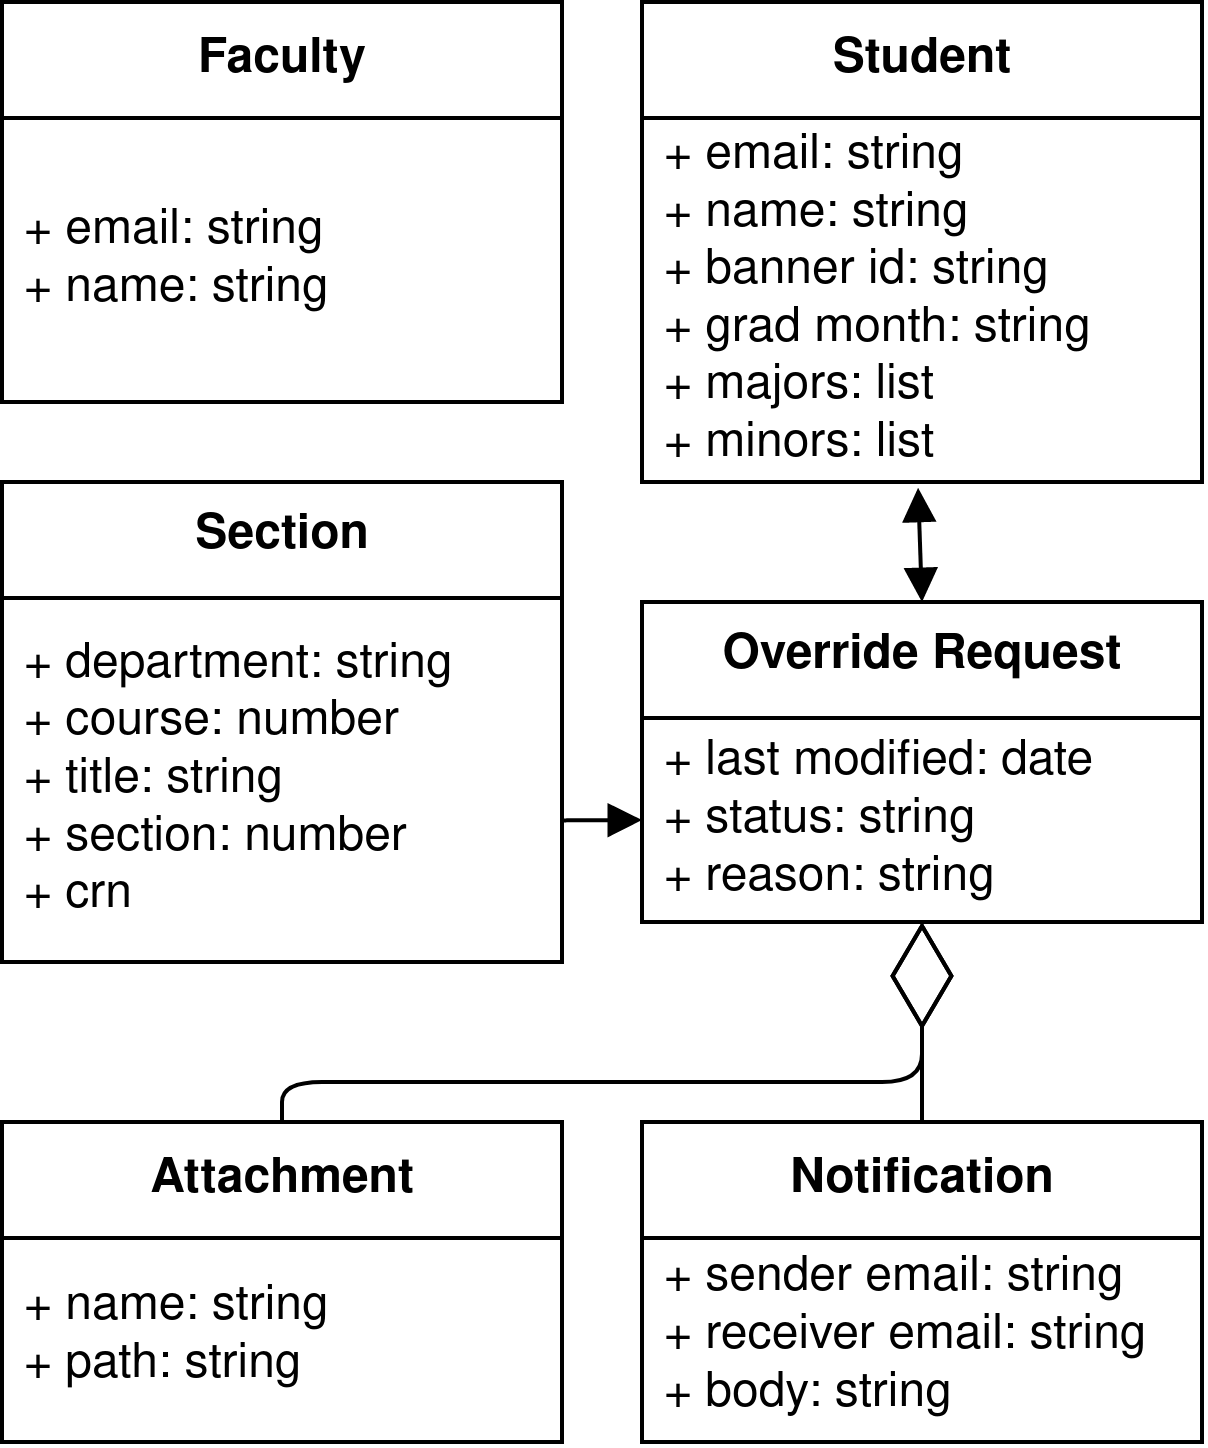
\includegraphics[width=\textwidth]{assets/database_classes.png}
\end{minipage}
\end{frame}

\section{Logic Progress}
\begin{frame}
  \frametitle{Logic Progress}

\begin{itemize}
    \item Took charge in the process that takes the request from the front-end and returns appropriate response from the system's database.
    \item Necessary to make sure that the communications between front-end and database could be faster and more convenient.
    \item The communication between the two parts was done through the use of API calls.
\end{itemize}

\end{frame}

\begin{frame}
    \frametitle{Logic Progress --- API}

\begin{itemize}
    \item Front-end requests certain data with required parameters (i.e. information) to the API.
    \item The API checks if the given request is valid.
    \begin{itemize}
        \item Returns error message if not.
    \end{itemize}
    \item The API gets the required data from database.
    \item Then returns the data back to the front-end.
\end{itemize}

\end{frame}

\section{Front-End Progress}
\begin{frame}
  \frametitle{Front-End Progress}

  

\end{frame}

\section{Demo}
\sectiontitle{Demo}

\section{}
\maketitle

\end{document}
